\documentclass{article}
\usepackage[margin=0.65in]{geometry}
\usepackage{enumitem}
\usepackage{graphicx}
\usepackage{hyperref}
\usepackage{titlesec}
\usepackage{xcolor}
\hypersetup{hidelinks}
\setlist[itemize]{leftmargin=1.5em,topsep=2pt,itemsep=1pt,parsep=0pt,partopsep=0pt}
\titlespacing*{\section}{0pt}{1.2ex}{0.6ex}
\setlength{\parindent}{0pt}
\setlength{\parskip}{0.5em}
\setlength{\textfloatsep}{8pt}
\setlength{\intextsep}{6pt}
\setlength{\abovecaptionskip}{4pt}
\setlength{\belowcaptionskip}{0pt}
\makeatletter
\renewcommand{\maketitle}{%
    \begin{center}
        {\Large\bfseries \@title\par}\vspace{0.3em}
        {\normalsize \@author\par}\vspace{0.2em}
        {\small \@date\par}
    \end{center}\vspace{0.4em}
}
\makeatother
% HJNotes-Tags: AI Infra, SGLang, FlashAttention, PagedAttention, RadixAttention
% HJNotes-Summary: Notes after reading 4 important papers about attention algorithm/system.
\title{Attention Inference Algorithm}
\author{HJ}
\begin{document}
\maketitle

\section{Introduction}
These notes survey some papers on attention inference.

Ideally, an attention kernel computes the current tile in on-chip SRAM while all other tiles (including the KV cache) are staged in HBM. Each paper attacks one side of this picture:
\begin{itemize}
    \item \textbf{FlashAttention} handles the compute side: an SRAM-aware kernel that keeps the working tile on chip and avoids materializing the full $N\times N$ attention matrix in HBM.
    \item \textbf{PagedAttention} handles the memory side: the KV cache is stored as non-contiguous pages behind a block table, removing fragmentation. Note that vLLM's scheduler is still first-come-first-served (FCFS); paging is PagedAttention's own contribution, not scheduling.
    \item \textbf{RadixAttention} builds on PagedAttention's paging and adds two things: prefix reuse through a radix tree with LRU eviction, and cache-aware scheduling (longest-prefix-first over the KV-cache tree) that replaces FCFS.
\end{itemize}

\begin{figure}[!ht]
    \centering
    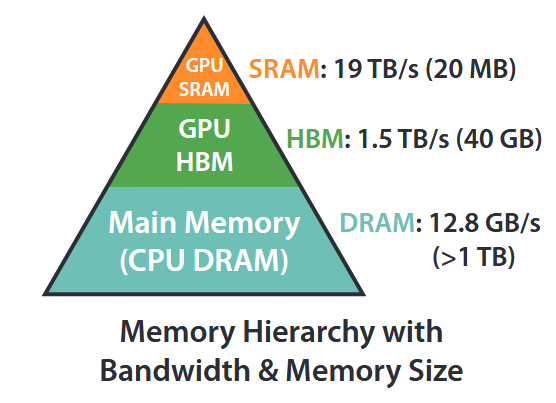
\includegraphics[width=\linewidth,height=0.16\textheight,keepaspectratio]{memory_hierachy_of_CPU_and_GPU.png}
    \caption{Memory hierarchy of CPU and GPU (SRAM vs HBM).}
\end{figure}

\section{FlashAttention}
\subsection{Compute-bound \& Memory-bound Operators}
\begin{itemize}
    \item \textbf{Compute-bound}: High arithmetic intensity. GEMM (matrix multiply) --- moves $O(n^2)$ data but performs $O(n^3)$ FLOPs, so arithmetic intensity grows with $n$.
    \item \textbf{Memory-bound}: Runtime is limited by memory bandwidth. softmax / dropout / element-wise ops --- they move $O(n)$ data while doing only $O(n)$ FLOPs, so they spend most of their time waiting on memory.
\end{itemize}
\underline{Attention is memory-bound}: $S = QK^\top$ and $P = \mathrm{softmax}(S)$ must be written to and read back from HBM. FlashAttention's contribution is keeping $S, P$ in SRAM instead of materializing them in HBM, thereby reducing HBM traffic.

\subsection{SRAM-awareness Tiling in v1}
Instead of materializing $S$ and $P$ in HBM, FlashAttention tiles $Q, K, V$ into blocks that fit in on-chip SRAM, computes each block's attention statistics there, and only writes the final output $O$ back to HBM. This reduces HBM traffic --- the tiles still move between SRAM and HBM, but the huge $N\times N$ intermediates never do.

\begin{figure}[!ht]
    \centering
    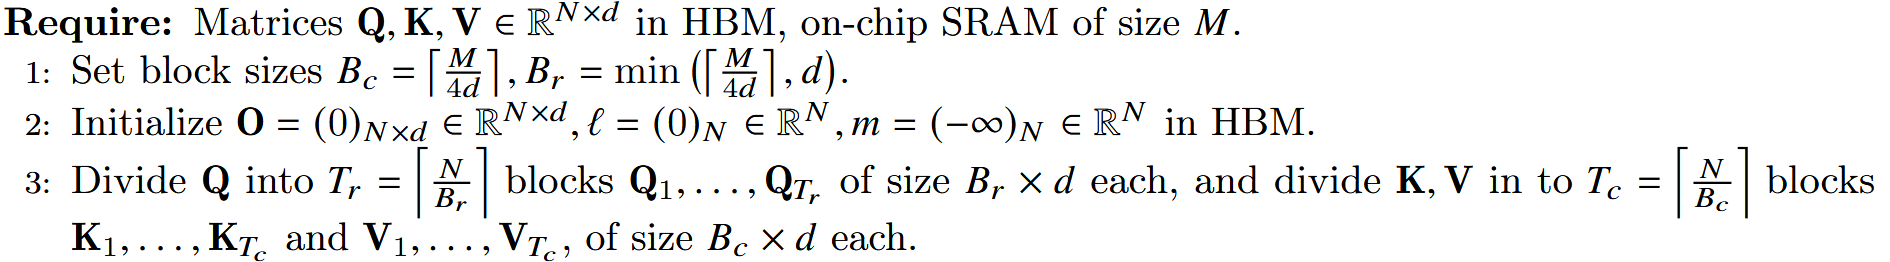
\includegraphics[width=\linewidth,height=0.52\textheight,keepaspectratio]{v1_tiling.png}
    \caption{FlashAttention v1 SRAM tiling: Q, K, V blocks are computed on chip.}
\end{figure}

\begin{itemize}
    \item \textcolor{blue}{\textbf{Why 4?}} A tile of $Q$, $K$, $V$, and $O$ must all sit in SRAM at once, so each block is bounded by roughly $M/4d$ (with $M$ the SRAM size and $d$ the head dimension).
    \item \textcolor{blue}{\textbf{Why $\min(\cdot, d)$?}} Without a cap, $B_r B_c \approx (M/4d)^2$; keeping the score tile $S$ within a quarter of SRAM then requires $(M/4d)^2 < M/4$, i.e.\ $M < 4d^2$, which often fails.
\end{itemize}

\subsection{Reduce Axis Q in Forward}
For the outer reduction axis, v1 uses a KV scheme, while v2 uses Q scheme. The new scheme has two advantages:
\begin{itemize}
    \item \textbf{Performance}: fewer HBM accesses --- the output accumulator stays on chip and is written back once instead of once per $K,V$ block.
    \item \textbf{Interpretation}: decoding-friendly --- decoding only needs the single row of $Q$ for the new token.
\end{itemize}

\begin{figure}[!ht]
    \centering
    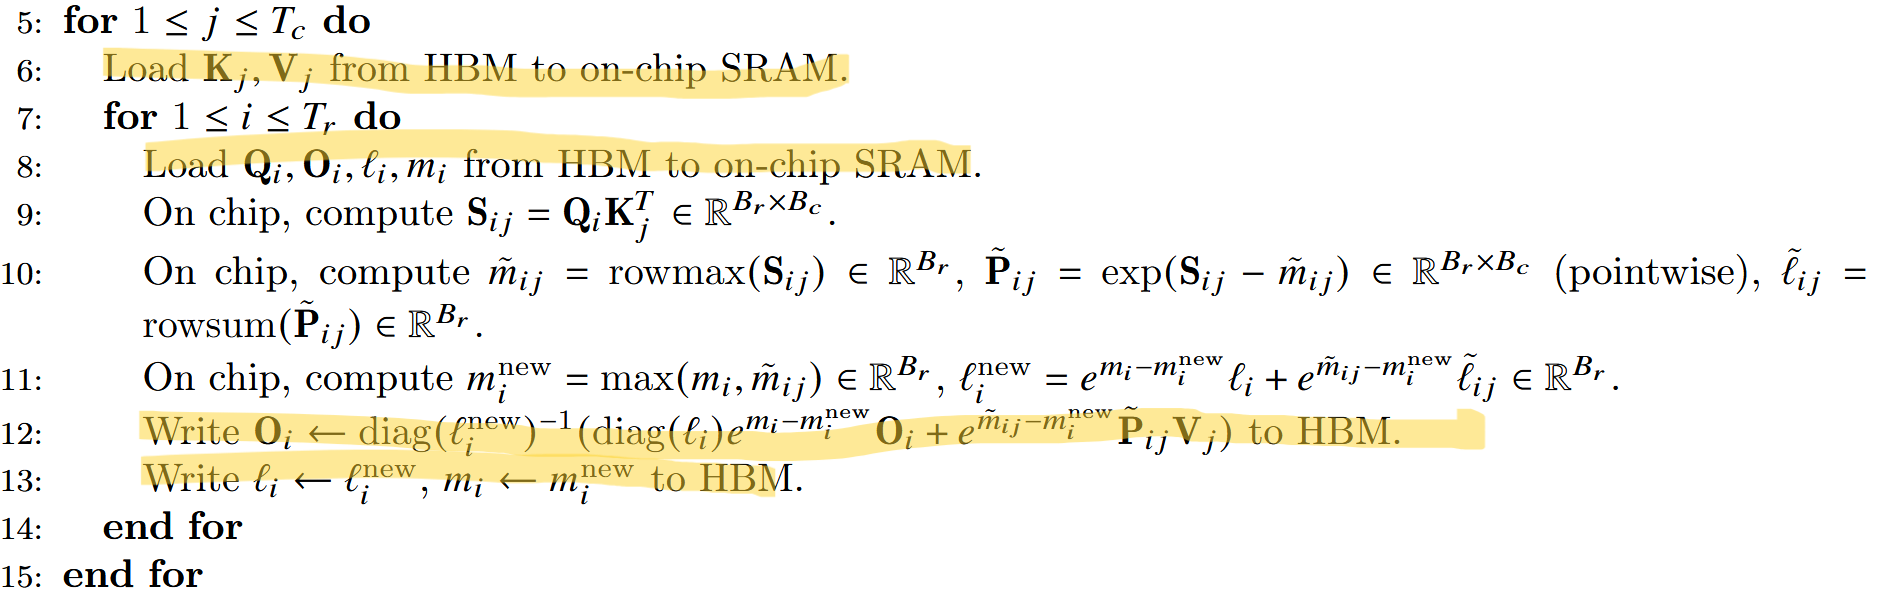
\includegraphics[width=\linewidth,height=0.52\textheight,keepaspectratio]{v1_algorithm.png}
    \caption{FlashAttention v1 forward algorithm (KV-split).}
\end{figure}

\begin{figure}[!ht]
    \centering
    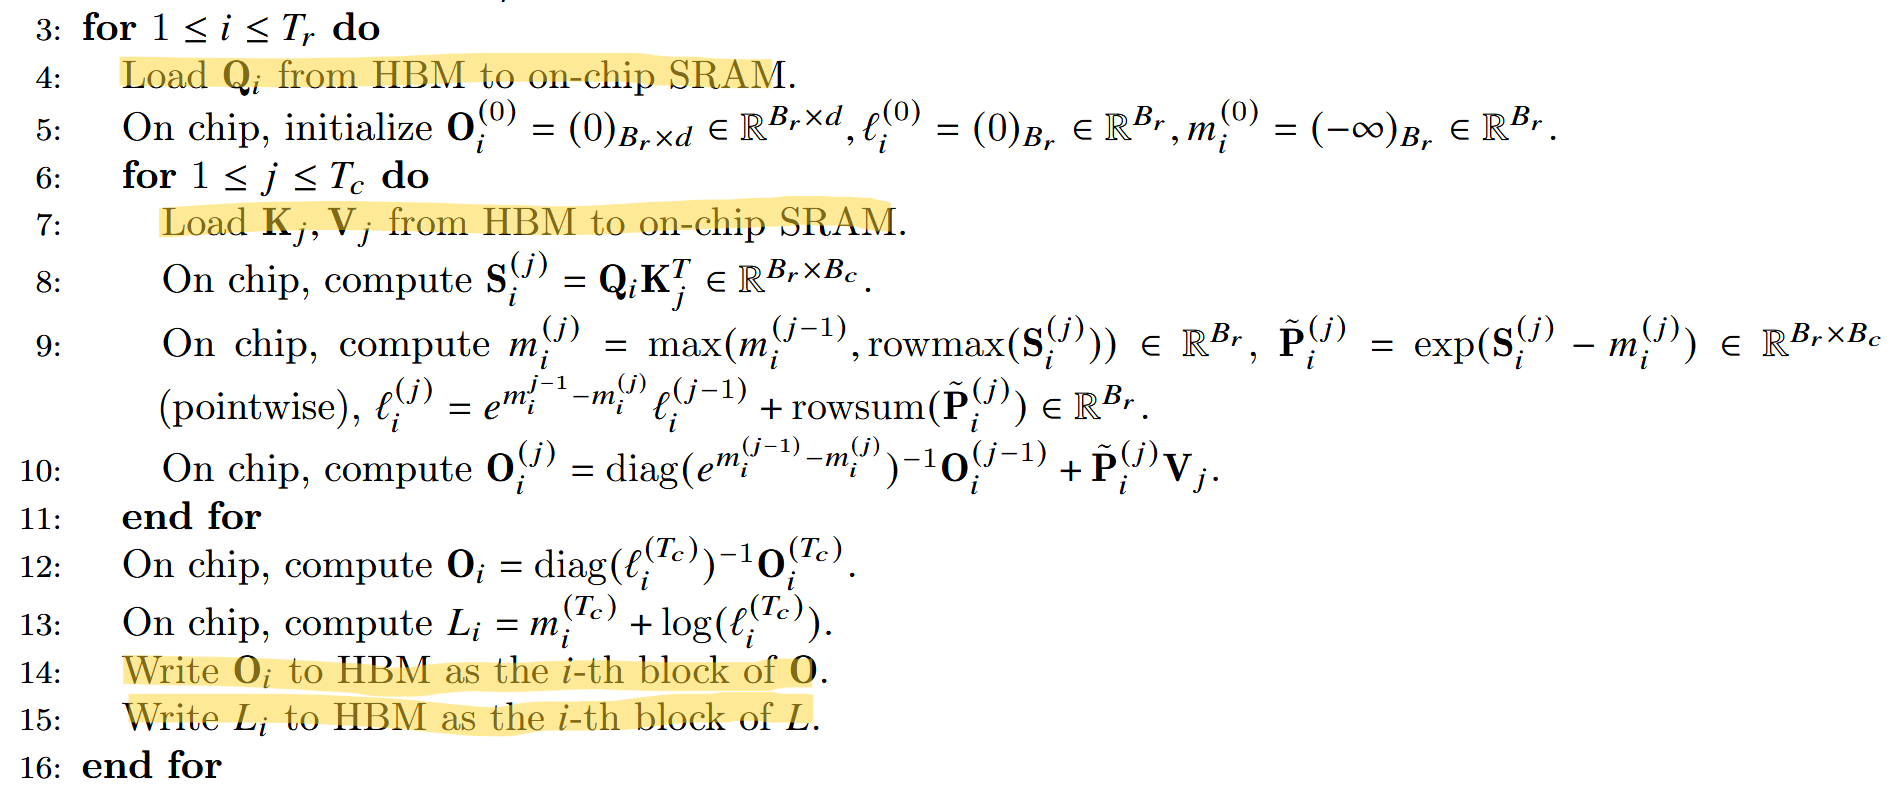
\includegraphics[width=\linewidth,height=0.52\textheight,keepaspectratio]{v2_algorithm.png}
    \caption{FlashAttention v2 forward algorithm (Q-split).}
\end{figure}

Triton puzzle 9 the Scalar FlashAttention can be seen as decoding once. is a good exercise for understanding how the v2 scheme works. Notation used below: $S$ is the accumulator over the whole row, $s$ is the local accumulator for the current tile.
\begin{figure}[!ht]
    \centering
    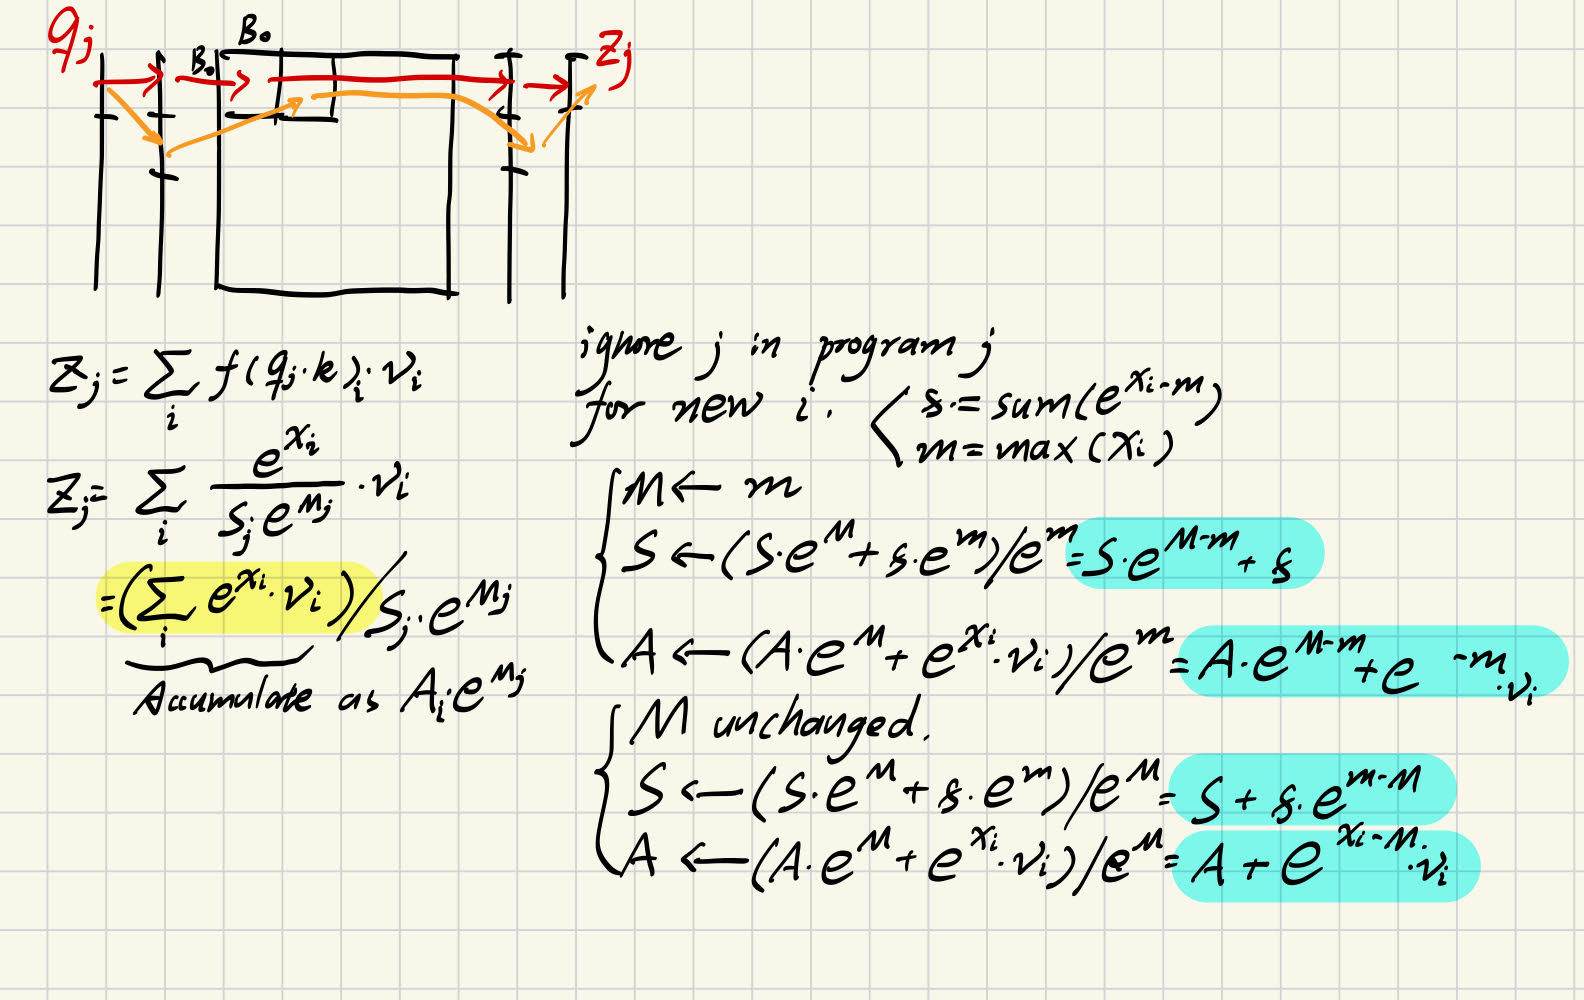
\includegraphics[width=\linewidth,height=0.47\textheight,keepaspectratio]{puzzle9.jpg}
    \caption{Triton puzzle 9 (FlashAttention forward).}
\end{figure}

\subsection{Reduce Axis KV in backward}
v2 still uses the KV-split scheme in the backward pass. The reason lies in the reduction axes: $dK$ and $dV$ share a reduction axis, while $dS$ has an independent one.
\begin{itemize}
    \item An outer reduction axis can be accumulated on chip and written back once
    \item An inner reduction axis changes at every step and must be written to HBM each time.
\end{itemize}

Hence $dK, dV$ are placed on the outer loop and $dS$ on the inner loop, minimizing HBM traffic.

\textcolor{blue}{Anyway, these are all about tradeoff.}

\begin{figure}[!ht]
    \centering
    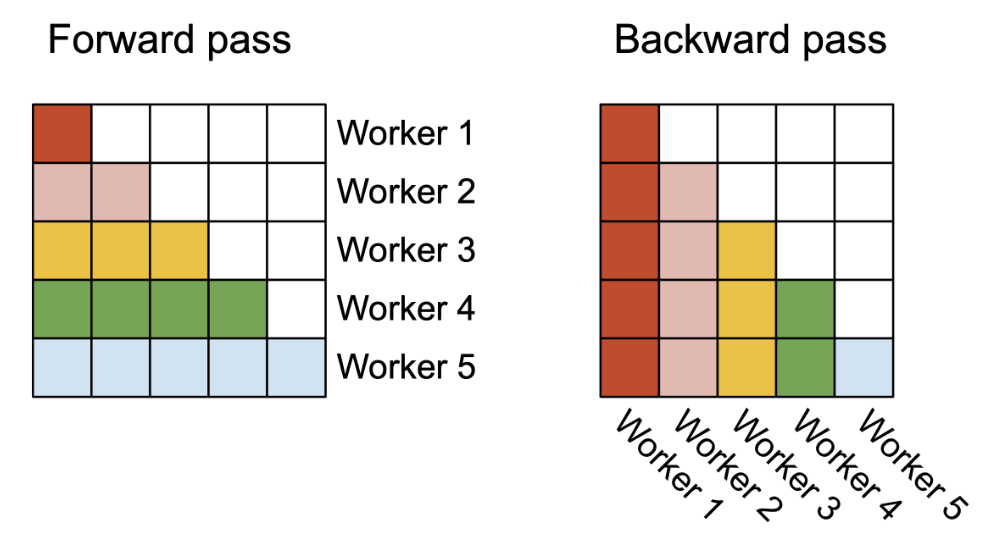
\includegraphics[width=\linewidth,height=0.23\textheight,keepaspectratio]{v2_reduce_axis_scheme.png}
    \caption{FlashAttention v2 backward reduce-axis scheme ($dK, dV$ outer, $dS$ inner).}
\end{figure}

\subsection{Causal Mask Minor Trick}
Because the causal mask adds $-\infty$ to masked positions, slightly fewer than half of the tiles can be skipped entirely (the strictly upper-triangular tiles), and only the diagonal tiles actually need the mask applied.

\section{PagedAttention}
\textcolor{red}{TODO?} Maybe won't do since I already take notes by zotero, and I believe those who need to read the paper won't need my notes, they could and would read original paper anyway.

\section{RadixAttention}
\textcolor{red}{TODO?}

\begin{thebibliography}{1}
\bibitem{flashattention} Tri Dao, Daniel Y. Fu, Stefano Ermon, Atri Rudra, Christopher Ré. \emph{FlashAttention: Fast and Memory-Efficient Exact Attention with IO-Awareness}. NeurIPS 2022.
\bibitem{flashattention2} Tri Dao. \emph{FlashAttention-2: Faster Attention with Better Parallelism and Work Partitioning}. 2023.
\bibitem{pagedattention} Woosuk Kwon et al. \emph{Efficient Memory Management for Large Language Model Serving with PagedAttention}. SOSP 2023.
\bibitem{sglang} Lianmin Zheng et al. \emph{SGLang: Efficient Execution of Structured Language Model Programs}. NeurIPS 2024.
\end{thebibliography}
\end{document}
